% flashcards-title: Three candidate graphs of candle length against time
% flashcards-desc: Three small graphs of length L in centimeters against time t in hours, labeled panel one, panel two, and panel three. Panel one shows a straight line rising from the origin. Panel two shows a straight line starting at twenty centimeters and falling to zero at ten hours. Panel three shows a curve starting at twenty centimeters that falls steeply at first and then levels off near six centimeters.
\documentclass[dvisvgm,tikz,border=8pt]{standalone}
\usepackage{tikz}
\usetikzlibrary{arrows.meta,calc,positioning}
\definecolor{DeckInk}{HTML}{172A3A}
\definecolor{DeckAccent}{HTML}{176B87}
\definecolor{DeckWarm}{HTML}{D97706}
\definecolor{DeckMuted}{HTML}{667784}
\definecolor{DeckPaper}{HTML}{F7FAFC}
\tikzset{
  every node/.style={font=\sffamily, text=DeckInk},
  object/.style={draw=DeckInk, line width=1.1pt, fill=DeckPaper},
  primary/.style={draw=DeckAccent, line width=1.5pt},
  boundary/.style={draw=DeckAccent, line width=1.5pt, dashed, rounded corners=6pt},
  guide/.style={draw=DeckMuted, line width=0.9pt, dashed},
  dimension/.style={{Stealth[length=3.2mm,width=2.2mm]}-{Stealth[length=3.2mm,width=2.2mm]}, draw=DeckWarm, line width=1.2pt},
  motion/.style={-{Stealth[length=3.5mm,width=2.5mm]}, draw=DeckAccent, line width=1.5pt, dashed},
}

\begin{document}
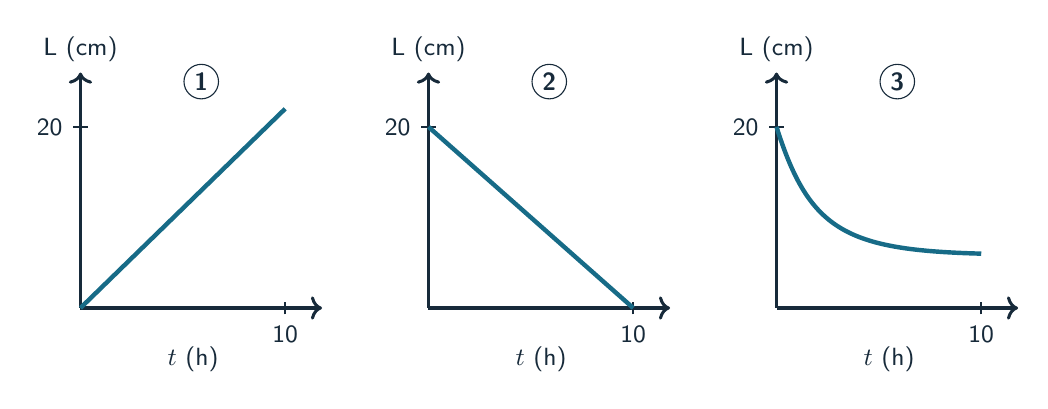
\begin{tikzpicture}[x=0.26cm, y=0.115cm]
  % Panel 1: straight line rising from the origin
  \begin{scope}
    \draw[object, ->] (0,0) -- (11.8,0);
    \node[below, font=\sffamily\small] at (5.5,-3.2) {$t$ (h)};
    \draw[object, ->] (0,0) -- (0,26) node[above, font=\sffamily\small] {L (cm)};
    \draw[DeckInk, line width=0.8pt] (10,-0.7) -- (10,0.7);
    \node[below, font=\sffamily\small] at (10,-0.9) {10};
    \draw[DeckInk, line width=0.8pt] (-0.35,20) -- (0.35,20);
    \node[left, font=\sffamily\small] at (-0.4,20) {20};
    \draw[DeckAccent, line width=1.6pt] (0,0) -- (10,22);
    \node[font=\sffamily\small\bfseries, draw=DeckInk, circle, inner sep=1.6pt]
      at (5.9,25) {1};
  \end{scope}
  % Panel 2: straight line from twenty centimeters down to zero at ten hours
  \begin{scope}[shift={(17,0)}]
    \draw[object, ->] (0,0) -- (11.8,0);
    \node[below, font=\sffamily\small] at (5.5,-3.2) {$t$ (h)};
    \draw[object, ->] (0,0) -- (0,26) node[above, font=\sffamily\small] {L (cm)};
    \draw[DeckInk, line width=0.8pt] (10,-0.7) -- (10,0.7);
    \node[below, font=\sffamily\small] at (10,-0.9) {10};
    \draw[DeckInk, line width=0.8pt] (-0.35,20) -- (0.35,20);
    \node[left, font=\sffamily\small] at (-0.4,20) {20};
    \draw[DeckAccent, line width=1.6pt] (0,20) -- (10,0);
    \node[font=\sffamily\small\bfseries, draw=DeckInk, circle, inner sep=1.6pt]
      at (5.9,25) {2};
  \end{scope}
  % Panel 3: curve falling steeply then leveling off near six centimeters
  \begin{scope}[shift={(34,0)}]
    \draw[object, ->] (0,0) -- (11.8,0);
    \node[below, font=\sffamily\small] at (5.5,-3.2) {$t$ (h)};
    \draw[object, ->] (0,0) -- (0,26) node[above, font=\sffamily\small] {L (cm)};
    \draw[DeckInk, line width=0.8pt] (10,-0.7) -- (10,0.7);
    \node[below, font=\sffamily\small] at (10,-0.9) {10};
    \draw[DeckInk, line width=0.8pt] (-0.35,20) -- (0.35,20);
    \node[left, font=\sffamily\small] at (-0.4,20) {20};
    \draw[DeckAccent, line width=1.6pt]
      (0,20) .. controls (1.6,8.5) and (3.4,6.4) .. (10,6);
    \node[font=\sffamily\small\bfseries, draw=DeckInk, circle, inner sep=1.6pt]
      at (5.9,25) {3};
  \end{scope}
\end{tikzpicture}
\end{document}
